\documentclass{proc}
\usepackage{url}
\usepackage{graphicx}
\begin{document}

\title{Exploring Trending Topic Bias in News vs. Social Media }

\author{Jonathan Galsurkar (jfg2150), Moorissa Tjokro (mmt2167), Nitesh Surtani (ns3148)}

\maketitle

\section{Abstract / Introduction}

\emph{1. What opportunities/changes that make this work useful and timely?
2. Why existing approaches fail to make use of these opportunities?
3. How do you propose to do better?
4. Why this problem is relevant to the course?
(1-2 sentences each)} 

Because of the constantly changing nature of the world and an increasing use of technology, having access to current events and up-to-date information has made people's lives more connected and visible in many ways. With social media growing as a platform to present information, it is crucial for news and media companies to bring accurate, unbiased, and edifying news both locally and around the world in a timely fashion. The news being talked about, however, may not represent what user of social media are talking about. Exploring biases between most trending topics on news and those being spoken about on social media would hence give both media companies and today's society the opportunity to observe the impact of information on people's interests and public opinions on news and various events throughout the world.

Currently, there is no specific approach or tool that effectively captures how different topics that are trending on news platforms differ from those on social media. With events happening in distant locations that can impact economies, political tides, and various commodities over the long term, the development of an exploration tool is important to understand how and what kind of information is being listened to and learned from.  

To maintain a quality standard of the accuracy and immediacy of news, the bias-trend platform can be improved by incorporating a real-time feature and trend comparison analysis. The analysis would allow users to see the topic biases between two platforms, and the real-time feature would keep users informed on what is currently happening in the world and how it is perceived through the two platforms.

This problem is relevant to the course because of the sheer amounts of data that will be worked it, making distributed systems and cloud computing an integral part of the project's success.

\section{One Sentence Summary}
\begin{quote}
\emph{Describe your project in one sentence, in other words, your hypothesis.}
\end{quote}

We will develop an exploration system which allows a user to intuitively compare trending topics in news platforms versus those on social media platforms.  We hypothesize that there is at least a moderate difference between topics presented in the news and topics spoken about on social media.

\section{Audience and Needs}
\begin{quote}
\emph{Who are the audiences for this project? 
How does it meet their needs? 
What happens if their needs remain unmet?}
\end{quote}

This project will prove to be a great asset to news, media, and any company that leverages consumer information.  Companies will be able to interactively see the differences between topics on the news versus topics actively spoken about on social media, allowing them to analyze the variance of discussions, understand what society cares about at the moment or in a given timeframe. News sources themselves can use our product to figure out how to improve their presentation of certain topics to get more traction from readers as well as infer patterns from topics not gaining traction.

\section{Approach}
\begin{quote}
\emph{What is your approach?
Why do you think it's a good approach and will be successful?}
\end{quote}



\begin{enumerate}

\item We will start with a set of manually selected trending topics and extract articles from News aggregator APIs (e.g. New York Times) and social media APIs (e.g. Twitter). We will attempt to capture the popularity of each topic, referred as a
\textit{Discussion Strength (DS)
\footnote{DS: Topics with high a Discussion Strength value are popular topics spoken about on social media, while those with low DS value are relatively less spoken about on social media.}}
using various metrics ranging from number of tweets and retweets to followers and responses, assuming the DS value for each article remains constant.

\item We will attempt to identify topic biases in Discussion Strength (DS) values of both news and social media platform through data visualizations and metrics analysis. This will give us understanding of parameters with higher significance and better DS values which may indicate correlation and causality of particular trends in topics on news and social media.

\item We will develop a clustering model which will form clusters of trending topics based on their DS. Assuming that there is
bias in the DS, we believe that different clusters will capture different categories of topics showing that some categories of topics
are over-spoken on social media than others.

\item We will implement a system to automatically scrape data from News and Social Media APIs and link the data of same trending topic
for these two platforms. The summarizer module will collect the statistics from the topics and store them in the database. Such information will be used directly for further analysis on the topics.

\item The search functionality will enable querying on the trending topics (or genre of topic) and finding whether that topic has been over-spoken or under-spoken. 

\item Later, we will try to scale the system in parallel to further fetch and process the data. 

\begin{figure}[t]
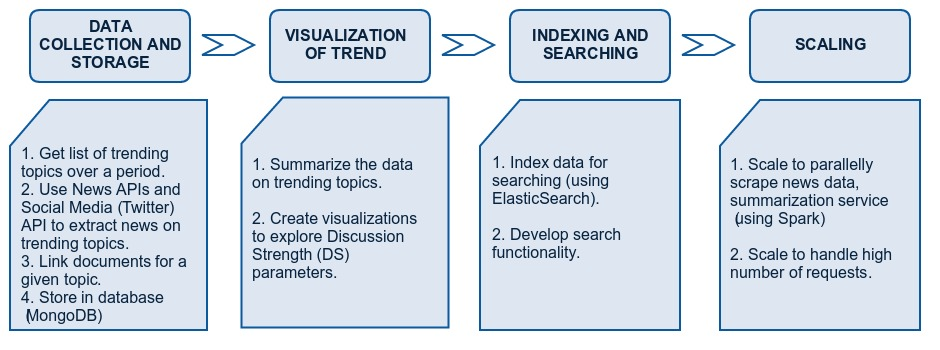
\includegraphics[width=9cm]{workflow.jpg}
\caption{Workflow of the project}
\end{figure}

\end{enumerate}

\section{(Best Case) Impact}
\begin{quote}
\emph{In the best-case scenario, what would be the impact statement (ideal outcome and conclusion) for this project?} 
\end{quote}

We can show that there is a discrepancy between trending topics being shared and spoken about on social media versus those presented on news platforms. This will in turn allow for analysis on topics of human interest as well as analysis of topics of disinterest on news platforms.

\section{Milestones}
\begin{quote}
\emph{List all major milestones for this project}
\end{quote}

\begin{enumerate}
  \item Gather news data into a structured format.
  \item Gather social media data into a structured format.
  \item Cluster/classify similar data into topics based on platform.
  \item Rank topics in clusters by popularity with associated examples.
  \item Develop functionality to search through the data.
  \item Develop functionality to visualize the data.
  \item Scale our system to handle a larger capacity of data at once.
\end{enumerate}

\section{Obstacles}
\begin{quote}
\emph{What are the major and minor obstacles that could happen? 
Note that major obstacles are situations where you would consider \textbf{killing} the project. 
Minor obstacles are things that would delay the project or increase the overall cost in energy, time, people, and money.}
\end{quote}

\subsection{Major obstacles} 

\begin{itemize}
    \item Assuming we have a way to store and access vast amount of the data that we gathered, we may not have access to the computing resources necessary to run real time analysis and visualizations
   on extremely large sets of data. We could of course do analysis over smaller time periods, which could reduce the impact of the project, through showing a bias for even smaller time periods is still a contribution. We may also
   have to rely on pre-computations which would make it difficult to present up to date information on very current topics.
\end{itemize}

\subsection{Minor obstacles}

\begin{itemize}
  \item We may not have access to the storage resources required to store years of news and social media data. One year of data alone can yield hundreds of gigabytes of data.
  \item We may not have access to  the "classes" of certain topics of news and social media data, depending on the APIs used, hence classifying the data may prove challenging and a clustering approach will be needed instead.
  \item Depending on the APIs available, we may not have access to data sets from certain social media or news platforms, thus possibly introducing slight bias to our results depending on our data sources.
\end{itemize}


\section{Additional Resources}
\begin{quote}
\emph{What additional resources do you need to complete this project?}
\end{quote}

\begin{itemize}
  \item Some computational time to run our optimizer algorithm to generate information from news and social media APIs.
  \item Access to a machine where we can install and run experiments, and possibly scale our system, using the current database prototype.
 \end{itemize}
 
\section{Literature Review}
\begin{quote}

\emph{List 5 major publications that are most relevant to this project, and how they are related.}
\end{quote}

\begin{itemize}
\item \emph{Background for the project:} This work does an extensive study on the Twitter trending topic~\cite{kwak2010twitter} and studies the 
temporal behavior and user participation on these topics. They work on the complete Twitter data comprising of 41.7 million
user profiles, 1.47 billion social relations, 4,262 trending topics, and 106 million tweets. \cite{hermida2012share}
works on exploring the popularity of news platform vs social media for consuming news.
 
\item \emph{Work the project relies and builds on: } \cite{tsagkias2011linking} does some interesting work 
on finding the social media utterances that implicitly reference the given news articles. The first module of our system builds on
the same approach on identifying the trending topics and querying Twitter to extract them.

\item \emph{Direct competitors: } We could not find any existing works which specifically focuses on exploring the relationship between
news and social media to study the usage behavior of trending topics.

\item \emph{Alternatives to achieve the broader goal: } There is no relevant prior work done we found on this topic.

 \end{itemize}


\section{Define Success}
\begin{quote}
\emph{When / How do you know if you have succeeded in this project?
In other words, what is the minimum finding that would make this project a success and publishable?}
\end{quote}

Simply developing an interactive platform that shows the variance between trending topics across social media and news platforms should be publishable, because a tool with this capability does not yet exist.

 \bibliographystyle{abbrv}
\begin{thebibliography}{99}

\bibitem{kwak2010twitter} Kwak, Haewoon and Lee, Changhyun and Park, Hosung and Moon, Sue, 
\emph{What is Twitter, a social network or a news media?}, Proceedings of the 19th international conference on World wide web,
2010.

\bibitem{tsagkias2011linking} Tsagkias, Manos and De Rijke, Maarten and Weerkamp, Wouter, 
\emph{Linking online news and social media}, Proceedings of the fourth ACM international conference on Web search and data mining,
2011.

\bibitem{bandari2012pulse} Bandari, Roja and Asur, Sitaram and Huberman, Bernardo A, 
\emph{The pulse of news in social media: Forecasting popularity}, arXiv preprint arXiv:1202.0332.
2012.

\bibitem{hermida2012share} Hermida, Alfred and Fletcher, Fred and Korell, Darryl and Logan, Donna, 
\emph{Share, like, recommend: Decoding the social media news consumer}, Journalism Studies. 2012.

\bibitem{newman} Newman, Nic, William H. Dutton, and Grant Blank. 
\emph{Social media in the changing ecology of news: The fourth and fifth estates in Britain.}
International Journal of Internet Science 7.1 (2012): 6-22.

\bibitem{marcel} Broersma, Marcel, and Todd Graham. 
\emph{Social media as beat: Tweets as a news source during the 2010 British and Dutch elections.}
Journalism Practice 6.3 (2012): 403-419.

\bibitem{wilma} Stassen, Wilma. 
\emph{Your news in 140 characters: exploring the role of social media in journalism.}
Global Media Journal-African Edition 4.1 (2010): 116-131.


\bibitem{weeks} Weeks, Brian E., and R. Lance Holbert. 
\emph{Predicting dissemination of news content in social media a focus on reception, friending, and partisanship.}
Journalism and Mass Communication Quarterly 90.2 (2013): 212-232.

\end{thebibliography}

\end{document}
